
\section{Resultados}
Tras ejecutar todos los pasos, todos los resultados obtenidos se irán guardando en la carpeta results. Como se han seguido una serie de pasos durante la investigación, en este apartado se irán mostrando los resultados de cada sección. 

Antes de hacer la investigación, leímos varios artículos para encontrar el número de proteínas del SARS-CoV-2. Las proteínas encontradas fueron las mostradas en la tabla. 

  

		\begin{table}[h!]
			\caption{Proteinas del SARS-CoV-2 usadas en la red}
			\begin{tabular}{cccc}
				\hline
				& Proteínas del covid  &   & \\ 
				\hline
				"NSP6" & "NSP1" & "NSP2" & "NSP5"\\
				"NSP7" & "NSP5" & "NSP8"  & "NSP9"\\
				"NSP11" & "NSP12" & "NSP13" & "NSP14"\\ 
				"NSP15" & "S" & "E" & "N"\\
				"M" & "ORF3a" & "ORF3b" & "ORF8"\\
				"ORF6" & "ORF7a" & "ORF9b" & "ORF9c"\\
                "ORF10" \\
				\hline
				\label{tab:ejemplo}
			\end{tabular}
		\end{table}

		
En los artículos venían que había 29 proteínas, pero que solo se utilizaron 26 de ellas. Por eso en los resultados, sólo hay 26. 
El fichero que contienen las proteínas las introducimos en STRING para encontrar el interactoma y tuvimos de resultado la siguiente red. 

		\begin{figure}[h!]
			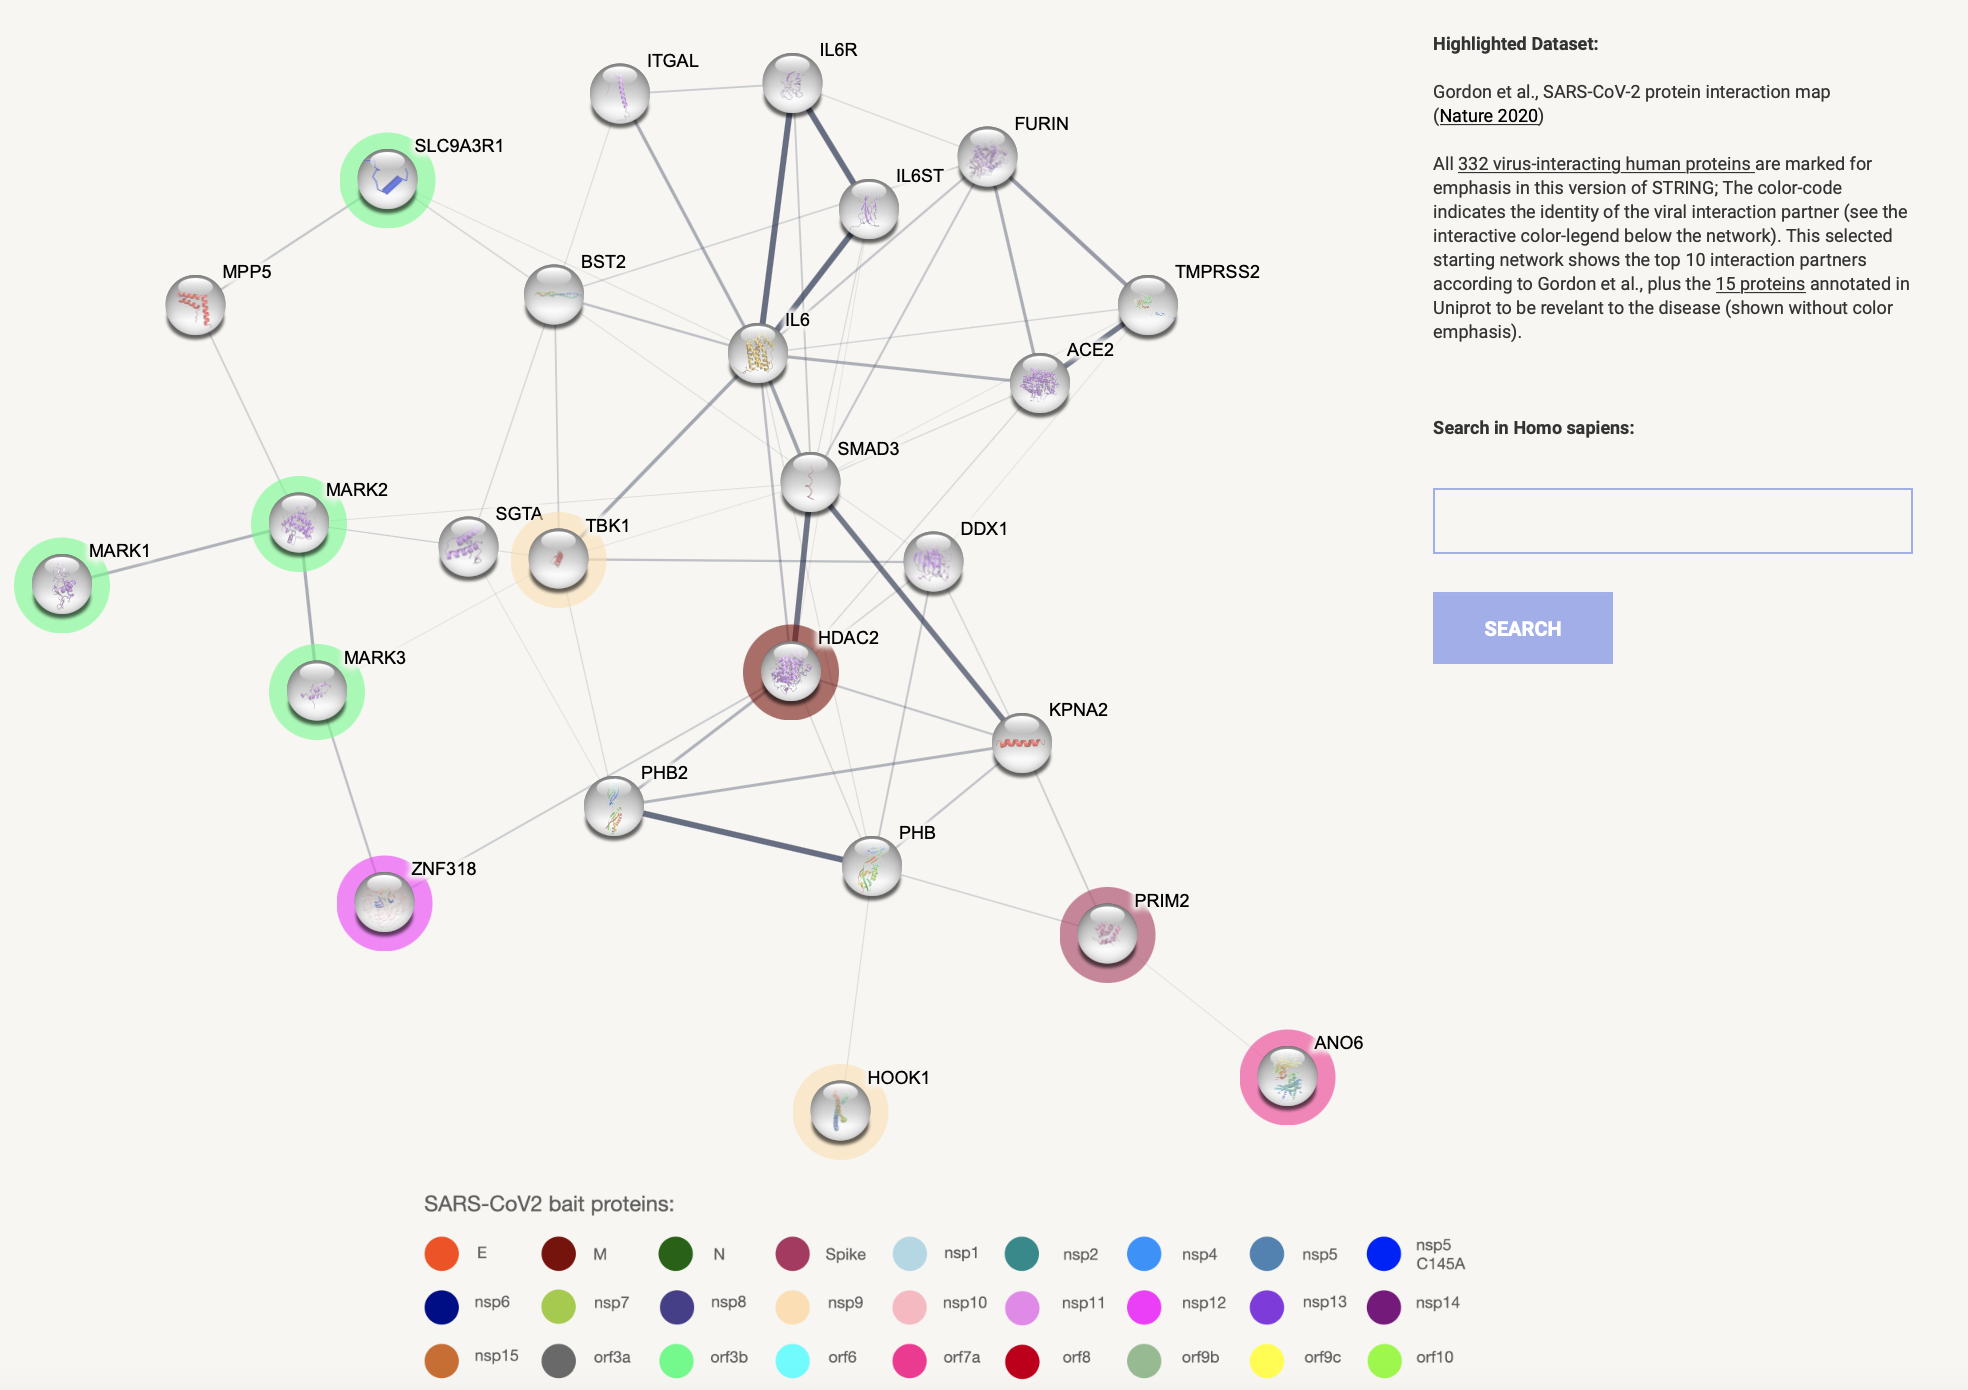
\includegraphics[width=0.8\textwidth]{figures/redinteractoma.jpg}
			\caption{Red proteinas humanas-proteinas SARS-CoV-2}
			\label{fig:cost_megabase}
		\end{figure}
		


En STRING obtuvimos 332 proteínas que interactuaban con las proteínas del SARS-CoV-2. Pero la red se divide en varios módulos, porque cada proteína del SARS-CoV-2 interactúa con un numero X de proteínas humanas. Por lo que, descargamos las 332 proteínas humanas para crear posteriormente una red entre ellas y elegir las que más fuerza de interacción tengan. 

Ejecutamos el fichero redString y nos da el resultado de 178 proteínas secundarias, que son las que usaremos para la búsqueda de los fármacos. 

		\begin{figure}[h!]
			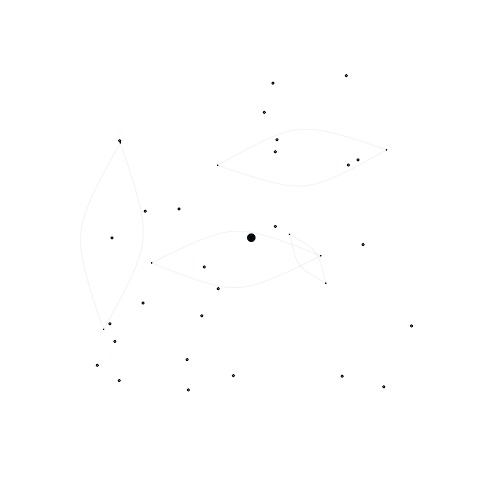
\includegraphics[width=0.6\textwidth]{figures/redsecundaria.jpeg}
			\caption{Red de proteinas huamnas}
			\label{fig:cost_megabase}
		\end{figure}
		
	\newpage

Todas esos genenames de proteinas las pasamos a Uniprot ID. 
		\begin{figure}[h!]
			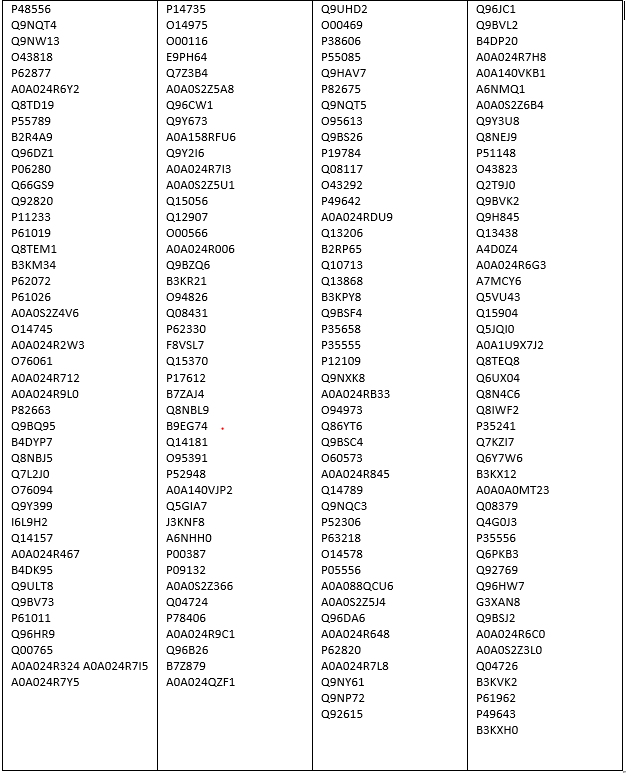
\includegraphics[width=0.9\textwidth]{figures/Captura1.PNG}
			\caption{Uniprot ID de las proteínas obtenidas en la red}
			\label{fig:cost_megabase}
		\end{figure}
		
Una vez obtenidos los UnitProt ID, buscamos los fármacos en la base de datos ChEMBL. Tras obtener loas datos de los fármacos tanto para la fase de aprobación como para la experimental, se realiza una serie de gráficos. A continuación, vamos a mostrar dos gráficas, una donde serán los tipos de fármacos que se utilizan en ensayos ya aprobados y la otra grafica los tipos de los ensayos experimentales. 

Se obtienen alrededor de 43 fármacos de ensayos experimentales y unos 66 de fármacos en los ensayos aprobados. 

\newpage

		\begin{figure}[h!]
			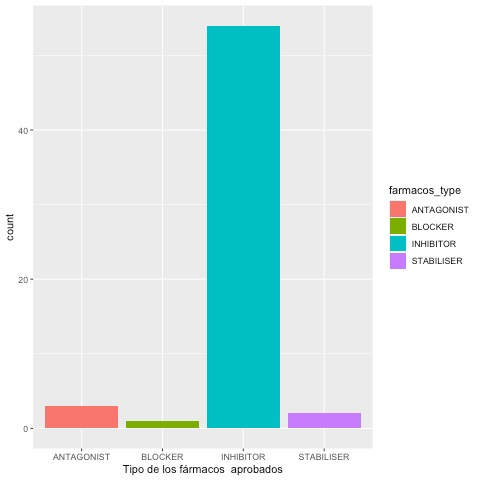
\includegraphics[width=0.7\textwidth]{figures/farmacosaprobados.jpeg}
			\caption{Grafica del tipo de fármacos aprobados}
			\label{fig:cost_megabase}
		\end{figure}
 


		\begin{figure}[h!]
			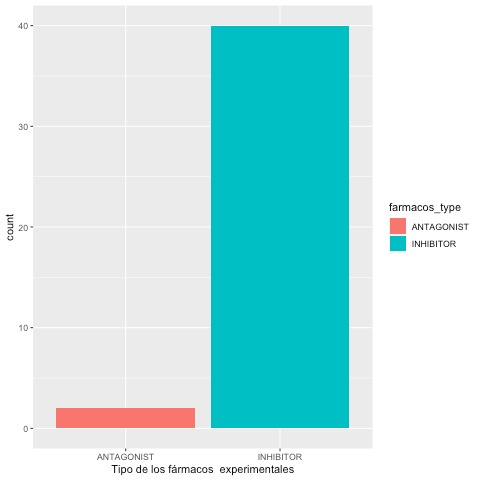
\includegraphics[width=0.7\textwidth]{figures/farmacosexperimentales.jpeg}
			\caption{Grafica del tipo de fármacos aprobados}
			\label{fig:cost_megabase}
		\end{figure}
Como observamos en esta primera grafica y en la segunda, la mayor parte de fármacos son de tipo inhibidor.

\newpage